\chapter{Method}

\begin{figure}[h]
\centering
\includegraphics[width=0.7\textwidth]{images/method_overview}
\caption{Overview of Crowd-Crossing Counting pipeline}
\label{fig:method_overview}
\end{figure}
In this chapter the proposed method for Crowd Crossing Counting is explained. As shown in figure \ref{fig:method_overview}, the full pipeline of prediction is based in two stages. First we predict both the density map and the velocity map, then we use these maps to predict the Crowd-Crossing Count. In section \emph{Velocity Map and Density Map} are the methods explained to train/predict both the velocity map and density map. In section \emph{LOI counting} the method is explained to predict the Crowd-Crossing Count based on those two intermediate maps.



\section{Velocity Map and Density Map}
Whereas earlier papers rely on velocity maps and density maps \cite{leibe_crossing-line_2016}, the amount of labelling required to train the models is high and creates an extra barrier for real world applications. To increase the usability of the method, an unsupervised velocity map estimation is used.

Training to predict both maps is being done in a paralel matter using a unified loss function described in equation \ref{eq:method_loss_total}. For the density loss, $L_c$, a traditional L2 loss is used (Figure \ref{eq:l2_loss}). For the velocity loss $L_v$, the photometric loss from figure \ref{eq:photometric_loss} \cite{Yu2016, Janai2018} is used.

\begin{equation}
\label{eq:method_loss_total}
	L_{t} = L_{v} + \lambda \cdot L_{c}
\end{equation}

For training a pair of two consecutive frames is taken ($I_1$ and $I_2$) with a groundtruth $C$, which is the ground truth density of the first frame. The model optimizes to output $\widetilde{C}$ and $\widetilde{V}$.

\begin{equation}
\begin{aligned}
L_{c}=& \sum (C - \widetilde{C})^2
\end{aligned}
\label{eq:l2_loss}
\end{equation}

In figure \ref{eq:photometric_loss_psi}, $I_{2}^{w}$ and $I_{1}^{w}$ are warped images with the predicted velocity $\widetilde{V}$. $I_{2}^{w}$ is $I_{2}$ backward warped, so it optimizes to be equal to $I_1$ and $I_{1}^{w}$ is $I_1$ forward warped to optimize to $I_2$. $\psi$ is a robust loss function defined as in figure \ref{eq:photometric_loss_psi} with $\epsilon = 0.01$ and $q=0.4$ (As used in \cite{liu_ddflow_2019})

\begin{equation}
\begin{aligned}
L_{p}=& \sum \psi\left(I_{1}-I_{2}^{w}\right) +\sum \psi\left(I_{2}-I_{1}^{w}\right)
\end{aligned}
\label{eq:photometric_loss}
\end{equation}
\begin{equation}
\begin{aligned}
\psi(x) = (|x| + \epsilon)^q
\end{aligned}
\label{eq:photometric_loss_psi}
\end{equation}

As explained in the background chapter Velocity Map Prediction and Density Map prediction are two widely researched fields. Two separate models would be capable of predicting both the Velocity Map and Density Map accurately. However this produces extra overhead using two fully seperate models.

Therefore a new model is proposed which unifies both velocity map and density map prediction. Sharing a single encoder and two separate decoders for each task. Additionally several additions are made to the model to enhance the density map prediction using intermediate results of the velocity map decoder.

\subsection{Models}
\begin{figure}[h]
\centering
\includegraphics[width=0.8\textwidth]{images/method_unified1}
\caption{Unified model}
\label{fig:unified_model}
\end{figure}
The proposed model is a multi-headed model with a shared encoder shown as in figure \ref{fig:unified_model} . The model uses the original PWCNet network \cite{sun_pwc-net_2018} as backbone. The proposed model shares the encoder and decoder of the PWCNet, but adds a second decoder to predict a density map as well, as shown in figure \ref{fig:unified_model}.


\subsubsection{PWCNet}
The PWCNet network is a small two frame input flow estimator, which at the time of publication was the best performing supervised flow estimator and to the best of our knowledge still the best performing two frame model currently published. The network uses a u-shaped network of 6 different levels. Each level uses warping (correlation between warped image and first image) and a cost volume (Fig \ref{fig:pwc_base}) to refine the estimated flow estimation. Finally a context network is used to further refine the output.

\begin{figure}[h]
\centering
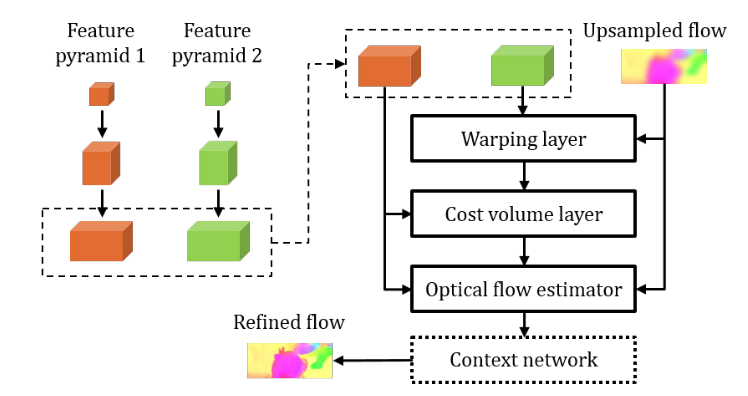
\includegraphics[width=0.7\textwidth]{images/pwcnet_approach}
\caption{PWCNet architecture}
\label{fig:pwc_base}
\end{figure}

\subsubsection{Density map decoder}
The density decoder contains of 5 upsampler modules with a final context network. Each upsampler module upsamples the output of the previous upsampler and concatenates it with the output of the encoder which are then smoothed with two regular conv-layers. The context module contains of 4 dilation layers with a respective dilation of 2,4,8,16 with a final layer to produce the density map.

\todo{Add figure to show the upsampler}

\subsubsection{Additional context}
The baseline density map decoder predicts a density only based on the first frame of the pair (Fig \ref{fig:unified_model}). However to the velocity map prediction, a lot of extra information is at our disposal to further enhance the density map prediction (Fig \ref{fig:enhanced_model}). Several further enhancements will be tested in this thesis:
\begin{itemize}
	\item Positional information, by adding using the encoder information of frame 2
	\item Flow information, by adding the raw cost volume of the flow estimator to the density decoder
	\item Warped information, by adding the warped positional information to the decoder
\end{itemize}

\begin{figure}[h]
\centering
\includegraphics[width=0.8\textwidth]{images/method_flow}
\caption{Flow enhanced model}
\label{fig:enhanced_model}
\end{figure}



\section{LOI counting}
The second stage merges both the velocity map and density map into two line crossing numbers. For our approach the main idea of \cite{leibe_crossing-line_2016} is taken (Explained in background) with extra smoothing to reduce the amount of outliers.

\label{sec:pixel_level}
We define $v_{perp}$ (White arrow in figure \ref{fig:loi_example}) as the normalized directional vector perpendicular to the LOI (Two solutions are perpendicular on the LOI and this defines sides 1 and 2 of the LOI counting). Then we define the collection of the pixels on the left side of the LOI and inside the LOI area as $M_1$ (side 1) and the pixels on the right side (side 1 and inside the LOI area) as $M_2$.
\todo{Add more visual description in same image as figure 2.3, explain that this assumption of left/right is without losing generality}

The velocity towards the LOI is then defined as the dot-product of $V_t$ and $v_{perp}$ (Equation \ref{eq:v_proj}).

\todo{Use two methods, smoothed one and non smoothed one (Zhao). Non-smoothed in background?}

\begin{equation}
	Q_t(p) = V_t(p) \cdot v_{perp}
	\label{eq:v_proj}
\end{equation}


\begin{equation}
\begin{aligned}
	c_{1,t} =& \sum_{\{p \in M_1 | Q_t(p) > 0\}} C_t(p) \cdot \frac{Q_t(p)}{d}\\
	c_{2,t} =& \sum_{\{p \in M_2 | Q_t(p) < 0\}} C_t(p) \cdot \frac{-Q_t(p)}{d}
\end{aligned}
\label{eq:pixel_cross}
\end{equation}

Then the LOI count on timestep $t$ is defined in equation \ref{eq:pixel_cross}. Where $\frac{Q_t(p)}{d}$ defines the percentage that the density on the specific pixel has crossed the LOI area. Lastly we can sum the count over a timespan into a single count for each side.

\subsection{Realigning}
In \cite{leibe_crossing-line_2016} a supervised method of aligning the velocity map and density map is used. However due to the unsupervised prediction of the velocity map in this thesis it is not possible to use this alignment. As shown in figure \ref{fig:maxing} this misalignment is an huge issue when multiplying the velocity map and density map in a pixel-wise matter. The blobs predicted in the density map are often much bigger than the flow of the pedestrian predicted. Additionally, for several Crowd datasets the tagging of the pedestrian is done on the head, which is why the blobs are ofter predicted over the head of the pedestrian.

To tackle this misalignment problem we propose an expanding method by applying a maxing filter on the flow estimation. This maxing filter takes the local maximum value in a surrounding of each pixel. Looking at figure \ref{fig:maxing} this helps to cover a lot of misaligned density maps and flow maps. To optimize for heads on the top side of the pedestrian, the maxing filter is focused on the bottom side of the selected pixel. Maximum values above the pixel are ignored.

\begin{figure}[h]
\centering
\includegraphics[width=1.0\textwidth]{images/compare_maxing}
\caption{On the right a non-maxed flow estimation and on the right the flow estimation with maxing filter applied}
\label{fig:maxing}
\end{figure}
\todo{V2, better labelling the dots in the figure, separating the figure description}
